%% LaTeX-Beamer template for KIT design
%% by Erik Burger, Christian Hammer
%% title picture by Klaus Krogmann
%%
%% version 2.1
%%
%% mostly compatible to KIT corporate design v2.0
%% http://intranet.kit.edu/gestaltungsrichtlinien.php
%%
%% Problems, bugs and comments to
%% burger@kit.edu




\documentclass[18pt]{beamer}

%% SLIDE FORMAT

% use 'beamerthemekit' for standard 4:3 ratio
% for widescreen slides (16:9), use 'beamerthemekitwide'

\usepackage{templates/beamerthemekit}
% \usepackage{templates/beamerthemekitwide}

%% TITLE PICTURE

% if a custom picture is to be used on the title page, copy it into the 'logos'
% directory, in the line below, replace 'mypicture' with the 
% filename (without extension) and uncomment the following line
% (picture proportions: 63 : 20 for standard, 169 : 40 for wide
% *.eps format if you use latex+dvips+ps2pdf, 
% *.jpg/*.png/*.pdf if you use pdflatex)

\titleimage{titelbild}

%% TITLE LOGO

% for a custom logo on the front page, copy your file into the 'logos'
% directory, insert the filename in the line below and uncomment it

%\titlelogo{blank}

% (*.eps format if you use latex+dvips+ps2pdf,
% *.jpg/*.png/*.pdf if you use pdflatex)

%% TikZ INTEGRATION

% use these packages for PCM symbols and UML classes
\usepackage{templates/tikzkit}
\usepackage{templates/tikzuml}

\usepackage{amsmath}
\usepackage{amssymb}
\usepackage{graphicx}

\usepackage{amsmath}

\usepackage{listings}
\usepackage{color}

\usepackage{tikz}
\usepackage{pgfplots}

\usepackage[utf8]{inputenc}
\usepackage[T1]{fontenc}

\usepackage{templates/subscript}

\usepackage{algorithmic}
\usepackage{listings}
\usepackage{color}
\usepackage[noeepic]{qtree}

\usepackage{pdfpages}
\usepackage{color, colortbl}
\usepackage{amssymb}

\usepackage{hyperref}
\newcommand*{\overlaynumber}{\number\beamer@slideinframe}
\tikzset{big node/.style={circle,fill=white,draw,inner sep=2pt,minimum size=0.5cm}}
\tikzset{little node/.style={circle,fill=white,draw,inner sep=1pt,minimum size=0.3cm}}
\tikzset{inv node/.style={circle,fill=white,draw=white,inner sep=2pt,minimum size=0.5cm}}
\tikzset{del node/.style={circle,fill=white,draw,inner sep=2pt,minimum size=1cm}}
\tikzset{unimp node/.style={circle,fill=white,draw=black!8,inner sep=2pt,minimum size=0.5cm}}
\tikzset{bigg node/.style={circle,fill=white,draw,inner sep=2pt,minimum size=0.68cm}}

\pgfdeclarelayer{bg}    % declare background layer
\pgfsetlayers{bg,main}

\lstdefinestyle{customc}{
	belowcaptionskip=1\baselineskip,
	breaklines=true,
	xleftmargin=\parindent,
	language=Java,
	showstringspaces=false,
	basicstyle=\footnotesize\ttfamily,
	keywordstyle=\bfseries\color{green!40!black},
	commentstyle=\itshape\color{purple!40!black},
	identifierstyle=\color{blue},
	stringstyle=\color{orange},
}

\lstdefinestyle{customasm}{
  belowcaptionskip=1\baselineskip,
  frame=L,
  xleftmargin=\parindent,
  language=[x86masm]Assembler,
  basicstyle=\footnotesize\ttfamily,
  commentstyle=\itshape\color{purple!40!black},
}

\definecolor{dkgreen}{rgb}{0,0.6,0}
\definecolor{gray}{rgb}{0.5,0.5,0.5}
\definecolor{mauve}{rgb}{0.58,0,0.82}

\lstset{escapechar=@} %,style=customc}

\lstset{emph={%  
		procedure%
	},emphstyle={\color{blue}\bfseries}%
}%

\lstset{frame=none,
	language=Java,
	aboveskip=3mm,
	belowskip=3mm,
	showstringspaces=false,
	columns=flexible,
	basicstyle={\small\ttfamily},
	numbers=left,
	numberstyle=\tiny,
	numbersep=5pt,
	numberstyle=\tiny\color{gray},
	keywordstyle=\color{blue},
	commentstyle=\color{dkgreen},
	stringstyle=\color{mauve},
	breaklines=true,
	breakatwhitespace=true,
	tabsize=3,
	xleftmargin=15pt,
}
% minimum width=3cm, text width=3cm,
\tikzstyle{io} = [trapezium, trapezium left angle=70, trapezium right angle=110,  minimum height=1cm, text centered, fill=blue!60, draw, double=blue, double distance =1pt]

\tikzstyle{rounded} = [rectangle, minimum width=3cm, minimum height=1cm, text centered, text width=3cm, fill=green!30, draw, double=green, double distance =1pt]

\tikzstyle{manuell} = [rectangle, minimum width=3cm, minimum height=1cm, text centered, text width=3cm, fill=red!30,draw, double=red, double distance =1pt]

\tikzstyle{r_box} = [rectangle, minimum width=7cm, minimum height=0.5cm, text width=7cm, text centered, align=center, draw, rounded corners=3pt]

\tikzstyle{r_box_min} = [rectangle, minimum width=3.3cm, minimum height=0.5cm, text width=3.3cm, text centered, align=center, draw, rounded corners=3pt, fill=blue!30]

\usepackage[absolute]{textpos}

\definecolor{LightCyan}{cmyk}{.5,0,.3,0}


% the presentation starts here

\title[Linear-Time Algorithm for Verifiying MST]{Linear-Time-Algorithm for Verifying Minimum Spanning Trees}
\author{Matthias Schimek}

\institute{Institute of Theoretical Informatics}

% Bibliography

\usepackage[citestyle=numeric,bibstyle=numeric,backend=biber]{biblatex}
\addbibresource{templates/lit.bib}
\bibhang1em
\nocite{*}

\date{18th July, 2017}

\begin{document}

% change the following line to "ngerman" for German style date and logos
\selectlanguage{english}

%title page
\begin{frame}
\titlepage
\end{frame}

\begin{frame}{MST-Verification}
	\begin{block}{MST-Verification}
	\emph{Given:} undirected Graph $G=(V,E)$, edge weights $\omega: E \rightarrow \mathbb{R}$ and spanning tree $T$ of $G$.
	\emph{Decide} whether $T$ is a MST of $G$.
	\end{block}
	\bigskip
	\pause
	\begin{block}{MST - Characterization}
		\centering{ $T$ is an $MST$ \\ $\Leftrightarrow$ \\
		$\forall$ nontree-edge $\{u,v\}$ with $(u,v)$-path $(e_1,\dots,e_l)$  in $T$:
		
		 $\omega(\{u,v\}) \ge \max(\omega(e_1),\dots,\omega(e_l))$.}
	\end{block}
\end{frame}
\begin{frame}{Tree-Path-Maxima-Problem}
	\begin{block}{Tree-Path-Maxima-Problem}
		\emph{Given:} 
		\begin{itemize}
			\item tree $T$ with real edge weights
			\item list of pairs of distinct vertices $(u,v)$
		\end{itemize}
		Determine for each pair ($u,v$) of the list  heaviest edge on $(u,v)$-path in $T$.
	\end{block}
	\pause
 	\begin{figure}
 		\centering
 		\begin{tikzpicture}[node distance=1.5cm]
 	%	\begin{scope}
 		\node (1) [little node] {};
 		\node (2) [little node, left of =1] {};
 		\node (3) [little node, below left of =2] {};
 		\node (4) [little node, above left of =2] {};
 		\node (5) [little node, left of =3] {};
 		\draw (5) +(150:0.5) node {$u$};
 		\node (6) [little node, below left of =3] {};
 		\node (7) [little node, below right of =1] {};
 		\node (8) [little node, below right of =7] {};
 		\node (9) [little node, above right of =1] {};
 		\node (10)[little node, right of =9] {};
 		\draw (10) +(30:0.5) node {$v$};
 		\node (11) [little node,below left of =1] {};
 		%\path (4) node (9) [little node] at +(-15:1.4) {};
 		
 		\only<1> {
 		\draw (11) -- (2) node[sloped,above,pos=0.5] {3};
 		\draw (1) -- (2) node[sloped,above,pos=0.5] {4};
 		\draw (1) -- (9) node[sloped,above,pos=0.5] {12};
 		\draw (9) -- (10) node[sloped,above,pos=0.5] {1};
 		\draw (1) -- (7) node[sloped,above,pos=0.5] {2};
 		\draw (2) -- (4) node[sloped,above,pos=0.5] {13};
 		\draw (2) -- (3) node[sloped,above,pos=0.5] {1};
 		\draw (3) -- (6) node[sloped,above,pos=0.5] {8};
 		\draw (3) -- (5) node[sloped,above,pos=0.5] {2};
 		\draw (7) -- (8) node[sloped,above,pos=0.5] {5};
 		}	
 		\only<2>{
 		\draw (11) -- (2) node[sloped,above,pos=0.5] {3};
 		\draw[color=blue] (1) -- (2) node[sloped,above,pos=0.5] {4};
 		\draw[color=blue] (1) -- (9) node[sloped,above,pos=0.5] {12};
 		\draw[color=blue] (9) -- (10) node[sloped,above,pos=0.5] {1};
 		\draw (1) -- (7) node[sloped,above,pos=0.5] {2};
 		\draw (2) -- (4) node[sloped,above,pos=0.5] {13};
 		\draw[color=blue] (2) -- (3) node[sloped,above,pos=0.5] {1};
 		\draw (3) -- (6) node[sloped,above,pos=0.5] {8};
 		\draw[color=blue] (3) -- (5) node[sloped,above,pos=0.5] {2};
 		\draw (7) -- (8) node[sloped,above,pos=0.5] {5};
 		}
 	 	\only<3>{
 	 		\draw (11) -- (2) node[sloped,above,pos=0.5] {3};
 	 		\draw[color=blue] (1) -- (2) node[sloped,above,pos=0.5] {4};
 	 		\draw[color=blue] (1) -- (9) node[sloped,above,pos=0.5] {{\color{red}12}};
 	 		\draw[color=blue] (9) -- (10) node[sloped,above,pos=0.5] {1};
 	 		\draw (1) -- (7) node[sloped,above,pos=0.5] {2};
 	 		\draw (2) -- (4) node[sloped,above,pos=0.5] {13};
 	 		\draw[color=blue] (2) -- (3) node[sloped,above,pos=0.5] {1};
 	 		\draw (3) -- (6) node[sloped,above,pos=0.5] {8};
 	 		\draw[color=blue] (3) -- (5) node[sloped,above,pos=0.5] {2};
 	 		\draw (7) -- (8) node[sloped,above,pos=0.5] {5};
 	 	}
 		
 		%\end{scope}
 		\end{tikzpicture}
 	\end{figure}
\end{frame}
\begin{frame}{Special-Tree-Path-Maxima-Problem (STPM)}
	\begin{block}{Tree-Path-Maxima-Problem}
		\emph{Given:} 
		\begin{itemize}
			\item {\color{blue}Full branching tree} $T$ with real edge weights
			\item list of pairs of distinct vertices $(u,v)$, \ $u$ is ancestor of $v$
		\end{itemize}
		Determine for each pair ($u,v$) a heaviest edge on $(u,v)$-path in $T$.
	\end{block}
	\pause
	\begin{figure}
		\centering
		\def\y{-0.5 cm}
		\def\z{-1.6cm}
		\def\a{-2.8cm}
		\begin{tikzpicture}[node distance=1.5cm]
			\only<1-2> {
					
				
			    %root
			    \draw node (0) [little node, fill=black] {};
			    %first line
			    \draw (-3,\y) node (1) [little node] {}; 
			    \draw (3, \y) node (2) [little node] {};
			    \draw (0) -- (1) node [sloped,above, pos=0.5] {3};
			    \draw (0) -- (2) node [sloped,above, pos=0.5] {11};
			    %second line
			    \draw (-4.5,\z) node (3) [little node] {};
			    \draw (-3.2,\z) node (4) [little node] {};
			    \draw (-1.9,\z) node (5) [little node] {};
			    \draw (1.9,\z) node (6) [little node] {};
			    \draw (4.5,\z) node (7) [little node] {};
			    \draw (1) -- (3) node [sloped,above, pos=0.5] {1};
			    \draw (1) -- (4) node [sloped,above, pos=0.5] {5};
			    \draw (1) -- (5) node [sloped,above, pos=0.5] {16};
			    \draw (2) -- (6) node [sloped,above, pos=0.5] {7};
			    \draw (2) -- (7) node [sloped,above, pos=0.5] {4};
	 		    %third line
	 		     \draw (-6.0,\a) node (8) [little node] {};
	 		    \draw (-4.8,\a) node (9) [little node] {};
	 		    \draw (-3.8,\a) node (10) [little node] {};
	 		    \draw (-3.0,\a) node (11) [little node] {};
	 		    \draw (-2.0,\a) node (12) [little node] {};
	 		    \draw (-1.0,\a) node (13) [little node] {};
	 		    \draw (1.0,\a) node (14) [little node] {};
	 		    \draw (2.0,\a) node (15) [little node] {};
	 		    \draw (3.0,\a) node (16) [little node] {};
	 		    \draw (4.0,\a) node (17) [little node] {};
	 		    \draw (4.9,\a) node (18) [little node] {};
	 		    
	 		    \draw (3) -- (8) node [sloped,above, pos=0.5] {6};
	 		    \draw (3) -- (9) node [sloped,above, pos=0.5] {7};
	 		    \draw (4) -- (10) node [sloped,above, pos=0.5] {1};
	 		    \draw (4) -- (11) node [sloped,above, pos=0.5] {2};
	 		    \draw (5) -- (12) node [sloped,above, pos=0.5] {8};
	 		    \draw (5) -- (13) node [sloped,above, pos=0.5] {6};
	 		    
	 		    \draw (6) -- (14) node [sloped,above, pos=0.5] {6};
	 		    \draw (6) -- (15) node [sloped,above, pos=0.5] {4};
	 		    \draw (6) -- (16) node [sloped,above, pos=0.5] {1};
	 		    \draw (7) -- (17) node [sloped,above, pos=0.5] {3};
	 		    \draw (7) -- (18) node [sloped,above, pos=0.5] {7};
	 		    %u,v	
	 		    \draw[color=white] (0) +(155:0.5cm) node (u) {u};
	 		    \draw[color=white] (13) +(10:0.5cm) node (v) {v};	
 		    }
 	    \only<3>{
 	    				
 	    	\draw (0) +(155:0.5cm) node (u) {u};
 	    	\draw (13) +(10:0.5cm) node (v) {v};		
 	    	%root
 	    	\draw node (0) [little node, fill=black] {};
 	    	%first line
 	    	\draw (-3,\y) node (1) [little node] {}; 
 	    	\draw (3, \y) node (2) [little node] {};
 	    	\draw[color = blue] (0) -- (1) node [sloped,above, pos=0.5] {3};
 	    	\draw (0) -- (2) node [sloped,above, pos=0.5] {11};
 	    	%second line
 	    	\draw (-4.5,\z) node (3) [little node] {};
 	    	\draw (-3.2,\z) node (4) [little node] {};
 	    	\draw (-1.9,\z) node (5) [little node] {};
 	    	\draw (1.9,\z) node (6) [little node] {};
 	    	\draw (4.5,\z) node (7) [little node] {};
 	    	\draw (1) -- (3) node [sloped,above, pos=0.5] {1};
 	    	\draw (1) -- (4) node [sloped,above, pos=0.5] {5};
 	    	\draw[color=blue] (1) -- (5) node [sloped,above, pos=0.5] {16};
 	    	\draw (2) -- (6) node [sloped,above, pos=0.5] {7};
 	    	\draw (2) -- (7) node [sloped,above, pos=0.5] {4};
 	    	%third line
 	    	\draw (-6.0,\a) node (8) [little node] {};
 	    	\draw (-4.8,\a) node (9) [little node] {};
 	    	\draw (-3.8,\a) node (10) [little node] {};
 	    	\draw (-3.0,\a) node (11) [little node] {};
 	    	\draw (-2.0,\a) node (12) [little node] {};
 	    	\draw (-1.0,\a) node (13) [little node] {};
 	    	\draw (1.0,\a) node (14) [little node] {};
 	    	\draw (2.0,\a) node (15) [little node] {};
 	    	\draw (3.0,\a) node (16) [little node] {};
 	    	\draw (4.0,\a) node (17) [little node] {};
 	    	\draw (4.9,\a) node (18) [little node] {};
 	    	
 	    	\draw (3) -- (8) node [sloped,above, pos=0.5] {6};
 	    	\draw (3) -- (9) node [sloped,above, pos=0.5] {7};
 	    	\draw (4) -- (10) node [sloped,above, pos=0.5] {1};
 	    	\draw (4) -- (11) node [sloped,above, pos=0.5] {2};
 	    	\draw (5) -- (12) node [sloped,above, pos=0.5] {8};
 	    	\draw[color=blue] (5) -- (13) node [sloped,above, pos=0.5] {6};
 	    	
 	    	\draw (6) -- (14) node [sloped,above, pos=0.5] {6};
 	    	\draw (6) -- (15) node [sloped,above, pos=0.5] {4};
 	    	\draw (6) -- (16) node [sloped,above, pos=0.5] {1};
 	    	\draw (7) -- (17) node [sloped,above, pos=0.5] {3};
 	    	\draw (7) -- (18) node [sloped,above, pos=0.5] {7};
 	    }
        \only<4>{
        	
        	\draw (0) +(155:0.5cm) node (u) {u};
        	\draw (13) +(10:0.5cm) node (v) {v};		
        	%root
        	\draw node (0) [little node, fill=black] {};
        	%first line
        	\draw (-3,\y) node (1) [little node] {}; 
        	\draw (3, \y) node (2) [little node] {};
        	\draw[color = blue] (0) -- (1) node [sloped,above, pos=0.5] {3};
        	\draw (0) -- (2) node [sloped,above, pos=0.5] {11};
        	%second line
        	\draw (-4.5,\z) node (3) [little node] {};
        	\draw (-3.2,\z) node (4) [little node] {};
        	\draw (-1.9,\z) node (5) [little node] {};
        	\draw (1.9,\z) node (6) [little node] {};
        	\draw (4.5,\z) node (7) [little node] {};
        	\draw (1) -- (3) node [sloped,above, pos=0.5] {1};
        	\draw (1) -- (4) node [sloped,above, pos=0.5] {5};
        	\draw[color=blue] (1) -- (5) node [sloped,above, pos=0.5] {{\color{red}16}};
        	\draw (2) -- (6) node [sloped,above, pos=0.5] {7};
        	\draw (2) -- (7) node [sloped,above, pos=0.5] {4};
        	%third line
        	\draw (-6.0,\a) node (8) [little node] {};
        	\draw (-4.8,\a) node (9) [little node] {};
        	\draw (-3.8,\a) node (10) [little node] {};
        	\draw (-3.0,\a) node (11) [little node] {};
        	\draw (-2.0,\a) node (12) [little node] {};
        	\draw (-1.0,\a) node (13) [little node] {};
        	\draw (1.0,\a) node (14) [little node] {};
        	\draw (2.0,\a) node (15) [little node] {};
        	\draw (3.0,\a) node (16) [little node] {};
        	\draw (4.0,\a) node (17) [little node] {};
        	\draw (4.9,\a) node (18) [little node] {};
        	
        	\draw (3) -- (8) node [sloped,above, pos=0.5] {6};
        	\draw (3) -- (9) node [sloped,above, pos=0.5] {7};
        	\draw (4) -- (10) node [sloped,above, pos=0.5] {1};
        	\draw (4) -- (11) node [sloped,above, pos=0.5] {2};
        	\draw (5) -- (12) node [sloped,above, pos=0.5] {8};
        	\draw[color=blue] (5) -- (13) node [sloped,above, pos=0.5] {6};
        	
        	\draw (6) -- (14) node [sloped,above, pos=0.5] {6};
        	\draw (6) -- (15) node [sloped,above, pos=0.5] {4};
        	\draw (6) -- (16) node [sloped,above, pos=0.5] {1};
        	\draw (7) -- (17) node [sloped,above, pos=0.5] {3};
        	\draw (7) -- (18) node [sloped,above, pos=0.5] {7};
        }
		\end{tikzpicture}
	\end{figure}
\end{frame}
\begin{frame}{MST-Verification $	\rightsquigarrow$ TPM-Problem}
	\begin{itemize}
		\item Graph $G=(V,E)$ and spanning tree $T$
		\item Is $T$ a MST? 
		\item [$\Leftrightarrow$] Check all non-tree edges $\{u,v\}$ against a heaviest edge on $(u,v)$-path
		
		\bigskip
		\pause
		\item [$\Rightarrow$] Reduces to TPM-Problem with 
		\begin{itemize}
			\item tree $T$
			\item List $L$ of queries $(u_i,v_i)$ and $|L| \le m$
		\end{itemize}
	\end{itemize}
\end{frame}
\begin{frame}{TPM-Problem $	\rightsquigarrow$ STPM-Problem}
	\begin{block}{Full-Branching Tree}
		Need {\color{blue} full-branching tree} with identical heaviest edge on each $(u_i,v_i)$-path
	\end{block}
	\begin{itemize}
		\item Boruvka-like construction of such a full-branching tree $T'$
		\begin{itemize}
			\item with $|T'| \le 2|T|$
			\item in $\mathcal{O}(|T|)$ time
		\end{itemize}
	\end{itemize}
	\bigskip
	\pause
	\begin{block}{Monotone path queries}
		SPTM only allows queries $(u_i,v_i)$ with $u_i$ ancestor of $v_i$.
	\end{block}
	\begin{itemize}
	\item Split up $(u_i,v_i)$-path into 2 monotone path $(u_i,z), (z, v_i)$,  \\ $z = \textup{{\color{blue}L}owest{\color{blue}C}ommon{\color{blue}A}ncestor}(u_i,v_i)$
	\item $LCA(u_i,v_i)$: $\mathcal{O}(|T|)$ preprocessing time, query in constant time
	\end{itemize}
\end{frame}
\begin{frame}{Algorithm for solving STPM}

	\begin{block}{STPM}
	 \begin{itemize}
	 	\item full-branching tree $T$
	 	\item List of $m$ monotone paths $(u_i,v_i)$
	 \end{itemize}
 	Determine a heaviest edge on each given path.
	\end{block}
	\bigskip
	\pause
	\begin{overprint}
		\onslide<1-2>
	\begin{itemize}
	\item  Several sets of vertices calculated by traversing $T$
	\item  Algorithm uses special {\color{blue}set operator} $\downarrow$:
	\[
		A \downarrow B := \{ b \in B \ | \ \exists a \in A: a < b \textup{ and no } b'\in B \textup{ with } a < b' < b \} 
	\]
	\item Informally: Each $a \in A$ 'picks' next larger $b \in B$ 
	\end{itemize}
	\onslide<3>
	\begin{itemize}
		\item  Several sets of vertices calculated by traversing $T$
		\item  Algorithm uses special {\color{blue}set operator} $\downarrow$:
		\[
		A \downarrow B := \{ b \in B \ | \ \exists a \in A: a < b \textup{ and no } b'\in B \textup{ with } a < b' < b \} 
		\]
		\item $A = \{1,3,6\}, \ B = \{1,2,3,4,5,6\}: \ \ A \downarrow B = \{2,4\}$ 
	\end{itemize}
	\end{overprint}
\end{frame}
\begin{frame}
	\begin{figure}
		\centering
		\def\a{-0.5 cm}
		\def\h{-0.6 cm}
		\def\b{-1.6cm}
		\def\c{-2.8cm}
		\def\d{-3.45cm}
		\def\leftdist{-7cm}
		\def\rightdist{0cm}
		\begin{tikzpicture}[node distance=1.5cm]
		\begin{overprint}
		\only<1>{
			%root
			\draw node (base) {};
			\draw  (base)  ++(-5cm,0cm) node (0) [little node, fill=black] {};
			\draw (0) ++(-1.5cm,\h) node (1) [little node]  {};
			\draw (1) ++(-1.2cm,\h) node (2) [little node]  {};
			\draw (2) ++(-0.8cm,\h) node (3) [little node]  {};
			\draw (3) ++(-0.7cm,\h) node (4) [little node]  {};
			\draw (4) ++(-0.6cm,\h) node (5) [little node]  {};
			\draw (5) ++(-0.5cm,\h) node (6) [little node, fill=red, opacity=.5]  {};
			\draw (6) ++(-0.4cm,\h) node (7) [little node]  {};
			
			\draw (0) +(2cm,\h) node (8) [little node] {};
			\draw (8) +(-0.8,\h) node (9) [little node] {};
			\draw (8) +(0.8,\h) node (10) [little node] {};
			\draw (9) +(-0.6,\h) node (11)  {$\dots$};
			\draw (9) +(0.45,\h) node (12)  {$\dots$};
			\draw (10) +(-0.4,\h) node (13)  {$\dots$};
			\draw (10) +(0.6,\h) node (14)  {$\dots$};
			\draw (1) ++(+1.2cm,\h) node (15)  {$\dots$};
			\draw (2) ++(+0.8cm,\h) node (16)   {$\dots$};
			\draw (3) ++(+0.7cm,\h) node (17)   {$\dots$};
			\draw (4) ++(+0.6cm,\h) node (18)   {$\dots$};
			\draw (5) ++(+0.5cm,\h) node (19)   {$\dots$};
			\draw (6) ++(+0.4cm,\h) node (20)  [little node] {};
			
			%additional edges
			\draw (0) -- (8) node [sloped,above,pos=0.5] {{\footnotesize 4}};
			\draw (8) -- (9) node [sloped,above,pos=0.7] {{\footnotesize 2}};
			\draw (8) -- (10) node [sloped,above,pos=0.5] {{\footnotesize 9}};
			\draw (9) -- (11) node [sloped,above,pos=0.5] {{\footnotesize 5}};
			\draw (9) -- (12) node [sloped,above,pos=0.5] {{\footnotesize 1}};
			\draw (10) -- (13) node [sloped,above,pos=0.5] {{\footnotesize 6}};
			\draw (10) -- (14) node [sloped,above,pos=0.5] {{\footnotesize 3}};
			
			\draw (1) -- (15) node [sloped,above,pos=0.7] {{\footnotesize 5}};
			\draw (2) -- (16) node [sloped,above,pos=0.5] {{\footnotesize 2}};
			\draw (3) -- (17) node [sloped,above,pos=0.5] {{\footnotesize 5}};
			\draw (4) -- (18) node [sloped,above,pos=0.5] {{\footnotesize 4}};
			\draw (5) -- (19) node [sloped,above,pos=0.5] {{\footnotesize 1}};
			\draw (6) -- (20) node [sloped,above,pos=0.5] {{\footnotesize 9}};
			
			% Gitter
			\draw[opacity=0] (0) +(\leftdist,0) node (0l) {0};
			\draw[opacity=0] (0) +(\rightdist,0) node (0r) {};
			\draw[opacity=0] (0) +(\leftdist,\h) node (1l) {1};
			\draw[opacity=0] (0) +(\rightdist,\h) node (1r) {};
			\draw[opacity=0] (0) +(\leftdist,2*\h) node (2l) {2};
			\draw[opacity=0] (0) +(\rightdist,2*\h) node (2r) {};
			\draw[opacity=0] (0) +(\leftdist,3*\h) node (3l) {3};
			\draw[opacity=0] (0) +(\rightdist,3*\h) node (3r) {};
			\draw[opacity=0] (0) +(\leftdist,4*\h) node (4l) {4};
			\draw[opacity=0] (0) +(\rightdist,4*\h) node (4r) {};
			\draw[opacity=0] (0) +(\leftdist,5*\h) node (5l) {5};
			\draw[opacity=0] (0) +(\rightdist,5*\h) node (5r) {};
			\draw[opacity=0] (0) +(\leftdist,6*\h) node (6l) {6};
			\draw[opacity=0] (0) +(\rightdist,6*\h) node (6r) {};
			\draw[opacity=0] (0) +(\leftdist,7*\h) node (7l) {7};
			\draw[opacity=0] (0) +(\rightdist,7*\h) node (7r) {};
			
			%depth
			%\foreach \x/\y/\z in {0l/0r/0,1l/1r/1,2l/2r/2,3l/3r/3,4l/4r/4,5l/5r/5,6l/6r/6,7l/7r/7}
			%{
			%	\begin{pgfonlayer}{bg}    % select the background layer
			%	\draw[dashed, color=gray, opacity=0.5] (\x) -- (\z); 
			%	\end{pgfonlayer}
			%}
			
			
			%edges
			\draw (0) -- (1) node [sloped,above,pos=0.5] {{\footnotesize 2}};
			\draw (1) -- (2) node [sloped,above,pos=0.7] {{\footnotesize 4}};
			\draw (2) -- (3) node [sloped,above,pos=0.5] {{\footnotesize 7}};
			\draw (3) -- (4) node [sloped,above,pos=0.5] {{\footnotesize 5}};
			\draw (4) -- (5) node [sloped,above,pos=0.5] {{\footnotesize 1}};
			\draw (5) -- (6) node [sloped,above,pos=0.5] {{\footnotesize 3}};
			\draw (6) -- (7) node [sloped,above,pos=0.5] {{\footnotesize 5}};
			
			
			
			%u_i,v_i
			\draw[opacity=0] (1) +(-0.8cm,0.2cm) node  {$u_1, u_3$};
			\draw[opacity=0] (3) +(-0.6cm,0.2cm) node  {$u_2$};
			\draw[opacity=0] (6) +(-0.6,0.2cm) node  {$v_1,v_2$};
			\draw[opacity=0] (7) +(-0.6,0cm) node  {$v_3$};
			%\draw[dashed, color=gray] (0l) -- (0r);
			
			% L-set
				\draw [dashed, color=gray, opacity=0] (7r) -- (7) node  [sloped,pos=0.5,opacity=0,color=black] {{\footnotesize$L = \{3\}$}};
			\draw [dashed, color=gray, opacity=0] (6r) -- (6) node  [sloped,pos=0.45,opacity=0,color=black] {{\footnotesize$L = \{1,2\}, D = \{1,3\},M = \{3,7\}$}};
			
		}	
		
		
		% ##########################2###############################
		
		\only<2> {
			%root
			\draw node (base) {};
			\draw  (base)  ++(-5cm,0cm) node (0) [little node, fill=black] {};
			\draw (0) ++(-1.5cm,\h) node (1) [little node]  {};
			\draw (1) ++(-1.2cm,\h) node (2) [little node]  {};
			\draw (2) ++(-0.8cm,\h) node (3) [little node]  {};
			\draw (3) ++(-0.7cm,\h) node (4) [little node]  {};
			\draw (4) ++(-0.6cm,\h) node (5) [little node]  {};
			\draw (5) ++(-0.5cm,\h) node (6) [little node, fill=red, opacity=.5]  {};
			\draw (6) ++(-0.4cm,\h) node (7) [little node]  {};
			
			\draw (0) +(2cm,\h) node (8) [little node] {};
			\draw (8) +(-0.8,\h) node (9) [little node] {};
			\draw (8) +(0.8,\h) node (10) [little node] {};
			\draw (9) +(-0.6,\h) node (11)  {$\dots$};
			\draw (9) +(0.45,\h) node (12)  {$\dots$};
			\draw (10) +(-0.4,\h) node (13)  {$\dots$};
			\draw (10) +(0.6,\h) node (14)  {$\dots$};
			\draw (1) ++(+1.2cm,\h) node (15)  {$\dots$};
			\draw (2) ++(+0.8cm,\h) node (16)   {$\dots$};
			\draw (3) ++(+0.7cm,\h) node (17)   {$\dots$};
			\draw (4) ++(+0.6cm,\h) node (18)   {$\dots$};
			\draw (5) ++(+0.5cm,\h) node (19)   {$\dots$};
			\draw (6) ++(+0.4cm,\h) node (20)  [little node] {};
			
			%additional edges
			\draw (0) -- (8) node [sloped,above,pos=0.5] {{\footnotesize 4}};
			\draw (8) -- (9) node [sloped,above,pos=0.7] {{\footnotesize 2}};
			\draw (8) -- (10) node [sloped,above,pos=0.5] {{\footnotesize 9}};
			\draw (9) -- (11) node [sloped,above,pos=0.5] {{\footnotesize 5}};
			\draw (9) -- (12) node [sloped,above,pos=0.5] {{\footnotesize 1}};
			\draw (10) -- (13) node [sloped,above,pos=0.5] {{\footnotesize 6}};
			\draw (10) -- (14) node [sloped,above,pos=0.5] {{\footnotesize 3}};
			
			\draw (1) -- (15) node [sloped,above,pos=0.7] {{\footnotesize 5}};
			\draw (2) -- (16) node [sloped,above,pos=0.5] {{\footnotesize 2}};
			\draw (3) -- (17) node [sloped,above,pos=0.5] {{\footnotesize 5}};
			\draw (4) -- (18) node [sloped,above,pos=0.5] {{\footnotesize 4}};
			\draw (5) -- (19) node [sloped,above,pos=0.5] {{\footnotesize 1}};
			\draw (6) -- (20) node [sloped,above,pos=0.5] {{\footnotesize 9}};
			
			% Gitter
			\draw[opacity=0] (0) +(\leftdist,0) node (0l) {0};
			\draw[opacity=0] (0) +(\rightdist,0) node (0r) {};
			\draw[opacity=0] (0) +(\leftdist,\h) node (1l) {1};
			\draw[opacity=0] (0) +(\rightdist,\h) node (1r) {};
			\draw[opacity=0] (0) +(\leftdist,2*\h) node (2l) {2};
			\draw[opacity=0] (0) +(\rightdist,2*\h) node (2r) {};
			\draw[opacity=0] (0) +(\leftdist,3*\h) node (3l) {3};
			\draw[opacity=0] (0) +(\rightdist,3*\h) node (3r) {};
			\draw[opacity=0] (0) +(\leftdist,4*\h) node (4l) {4};
			\draw[opacity=0] (0) +(\rightdist,4*\h) node (4r) {};
			\draw[opacity=0] (0) +(\leftdist,5*\h) node (5l) {5};
			\draw[opacity=0] (0) +(\rightdist,5*\h) node (5r) {};
			\draw[opacity=0] (0) +(\leftdist,6*\h) node (6l) {6};
			\draw[opacity=0] (0) +(\rightdist,6*\h) node (6r) {};
			\draw[opacity=0] (0) +(\leftdist,7*\h) node (7l) {7};
			\draw[opacity=0] (0) +(\rightdist,7*\h) node (7r) {};
			
			%depth
			\foreach \x/\y/\z in {0l/0r/0,1l/1r/1,2l/2r/2,3l/3r/3,4l/4r/4,5l/5r/5,6l/6r/6,7l/7r/7}
			{
				\begin{pgfonlayer}{bg}    % select the background layer
				\draw[dashed, color=gray, opacity=0.0] (\x) -- (\z); 
				\end{pgfonlayer}
			}
			
			
			%edges
			\draw (0) -- (1) node [sloped,above,pos=0.5] {{\footnotesize 2}};
			\draw (1) -- (2) node [sloped,above,pos=0.7] {{\footnotesize 4}};
			\draw (2) -- (3) node [sloped,above,pos=0.5] {{\footnotesize 7}};
			\draw (3) -- (4) node [sloped,above,pos=0.5] {{\footnotesize 5}};
			\draw (4) -- (5) node [sloped,above,pos=0.5] {{\footnotesize 1}};
			\draw (5) -- (6) node [sloped,above,pos=0.5] {{\footnotesize 3}};
			\draw (6) -- (7) node [sloped,above,pos=0.5] {{\footnotesize 5}};
			
			
			
			%u_i,v_i
			%u_i,v_i
			\draw (1) +(-0.8cm,0.2cm) node [color=blue] {$u_1, u_3$};
			\draw (3) +(-0.6cm,0.2cm) node [color=blue] {$u_2$};
			\draw (6) +(-0.6,0.2cm) node [color=blue] {$v_1,v_2$};
			\draw (7) +(-0.6,0cm) node [color=blue] {$v_3$};
			%\draw[dashed, color=gray] (0l) -- (0r);
			
			% L-set
			\draw [dashed, color=gray, opacity=0] (7r) -- (7) node  [sloped,pos=0.5,opacity=0,color=black] {{\footnotesize$L = \{3\}$}};
		\draw [dashed, color=gray, opacity=0] (6r) -- (6) node  [sloped,pos=0.45,opacity=0,color=black] {{\footnotesize$L = \{1,2\}, D = \{1,3\},M = \{3,7\}$}};
			
		}
	
	    % '#######################################3##################
		\only<3> {
			%root
			\draw node (base) {};
			\draw  (base)  ++(-5cm,0cm) node (0) [little node, fill=black] {};
			\draw (0) ++(-1.5cm,\h) node (1) [little node]  {};
			\draw (1) ++(-1.2cm,\h) node (2) [little node]  {};
			\draw (2) ++(-0.8cm,\h) node (3) [little node]  {};
			\draw (3) ++(-0.7cm,\h) node (4) [little node]  {};
			\draw (4) ++(-0.6cm,\h) node (5) [little node]  {};
			\draw (5) ++(-0.5cm,\h) node (6) [little node, fill=red, opacity=.5]  {};
			\draw (6) ++(-0.4cm,\h) node (7) [little node]  {};
			
			\draw[opacity=0] (0) +(2cm,\h) node (8) [little node] {};
			\draw[opacity=0] (8) +(-0.8,\h) node (9) [little node] {};
			\draw[opacity=0] (8) +(0.8,\h) node (10) [little node] {};
			\draw[opacity=0] (9) +(-0.6,\h) node (11)  {$\dots$};
			\draw[opacity=0] (9) +(0.45,\h) node (12)  {$\dots$};
			\draw[opacity=0] (10) +(-0.4,\h) node (13)  {$\dots$};
			\draw[opacity=0] (10) +(0.6,\h) node (14)  {$\dots$};
			\draw[opacity=0] (1) ++(+1.2cm,\h) node (15)  {$\dots$};
			\draw[opacity=0] (2) ++(+0.8cm,\h) node (16)   {$\dots$};
			\draw[opacity=0] (3) ++(+0.7cm,\h) node (17)   {$\dots$};
			\draw[opacity=0] (4) ++(+0.6cm,\h) node (18)   {$\dots$};
			\draw[opacity=0] (5) ++(+0.5cm,\h) node (19)   {$\dots$};
			\draw[opacity=0] (6) ++(+0.4cm,\h) node (20)  [little node] {};
			
			%additional edges
		
			
			% Gitter
			\draw[opacity=0] (0) +(\leftdist,0) node (0l) {0};
			\draw[opacity=0] (0) +(\rightdist,0) node (0r) {};
			\draw[opacity=0] (0) +(\leftdist,\h) node (1l) {1};
			\draw[opacity=0] (0) +(\rightdist,\h) node (1r) {};
			\draw[opacity=0] (0) +(\leftdist,2*\h) node (2l) {2};
			\draw[opacity=0] (0) +(\rightdist,2*\h) node (2r) {};
			\draw[opacity=0] (0) +(\leftdist,3*\h) node (3l) {3};
			\draw[opacity=0] (0) +(\rightdist,3*\h) node (3r) {};
			\draw[opacity=0] (0) +(\leftdist,4*\h) node (4l) {4};
			\draw[opacity=0] (0) +(\rightdist,4*\h) node (4r) {};
			\draw[opacity=0] (0) +(\leftdist,5*\h) node (5l) {5};
			\draw[opacity=0] (0) +(\rightdist,5*\h) node (5r) {};
			\draw[opacity=0] (0) +(\leftdist,6*\h) node (6l) {6};
			\draw[opacity=0] (0) +(\rightdist,6*\h) node (6r) {};
			\draw[opacity=0] (0) +(\leftdist,7*\h) node (7l) {7};
			\draw[opacity=0] (0) +(\rightdist,7*\h) node (7r) {};
			
			%depth
			\foreach \x/\y/\z in {0l/0r/0,1l/1r/1,2l/2r/2,3l/3r/3,4l/4r/4,5l/5r/5,6l/6r/6,7l/7r/7}
			{
				\begin{pgfonlayer}{bg}    % select the background layer
				\draw[dashed, color=gray, opacity=0.0] (\x) -- (\z); 
				\end{pgfonlayer}
			}
			
			
			%edges
			\draw (0) -- (1) node [sloped,above,pos=0.5] {{\footnotesize 2}};
			\draw (1) -- (2) node [sloped,above,pos=0.7] {{\footnotesize 4}};
			\draw (2) -- (3) node [sloped,above,pos=0.5] {{\footnotesize 7}};
			\draw (3) -- (4) node [sloped,above,pos=0.5] {{\footnotesize 5}};
			\draw (4) -- (5) node [sloped,above,pos=0.5] {{\footnotesize 1}};
			\draw (5) -- (6) node [sloped,above,pos=0.5] {{\footnotesize 3}};
			\draw (6) -- (7) node [sloped,above,pos=0.5] {{\footnotesize 5}};
			
			
			
			%u_i,v_i
			\draw (1) +(-0.8cm,0.2cm) node [color=blue] {$u_1, u_3$};
			\draw (3) +(-0.6cm,0.2cm) node [color=blue] {$u_2$};
			\draw (6) +(-0.6,0.2cm) node [color=blue] {$v_1,v_2$};
			\draw (7) +(-0.6,0cm) node [color=blue] {$v_3$};
			%\draw[dashed, color=gray] (0l) -- (0r);
			
			% L-set
				\draw [dashed, color=gray, opacity=0] (7r) -- (7) node  [sloped,pos=0.5,opacity=0,color=black] {{\footnotesize$L = \{3\}$}};
			\draw [dashed, color=gray, opacity=0] (6r) -- (6) node  [sloped,pos=0.45,opacity=0,color=black] {{\footnotesize$L = \{1,2\}, D = \{1,3\},M = \{3,7\}$}};
		}
	
	    % '#######################################4##################
	    \only<4-> {
	    	%root
	    	\draw node (base) {};
	    	\draw  (base)  ++(-5cm,0cm) node (0) [little node, fill=black] {};
	    	\draw (0) ++(-1.5cm,\h) node (1) [little node]  {};
	    	\draw (1) ++(-1.2cm,\h) node (2) [little node]  {};
	    	\draw (2) ++(-0.8cm,\h) node (3) [little node]  {};
	    	\draw (3) ++(-0.7cm,\h) node (4) [little node]  {};
	    	\draw (4) ++(-0.6cm,\h) node (5) [little node]  {};
	    	\draw (5) ++(-0.5cm,\h) node (6) [little node, fill=red, opacity=.5]  {};
	    	\draw (6) ++(-0.4cm,\h) node (7) [little node]  {};
	    	
	    	\draw[opacity=0] (0) +(2cm,\h) node (8) [little node] {};
	    	\draw[opacity=0] (8) +(-0.8,\h) node (9) [little node] {};
	    	\draw[opacity=0] (8) +(0.8,\h) node (10) [little node] {};
	    	\draw[opacity=0] (9) +(-0.6,\h) node (11)  {$\dots$};
	    	\draw[opacity=0] (9) +(0.45,\h) node (12)  {$\dots$};
	    	\draw[opacity=0] (10) +(-0.4,\h) node (13)  {$\dots$};
	    	\draw[opacity=0] (10) +(0.6,\h) node (14)  {$\dots$};
	    	\draw[opacity=0] (1) ++(+1.2cm,\h) node (15)  {$\dots$};
	    	\draw[opacity=0] (2) ++(+0.8cm,\h) node (16)   {$\dots$};
	    	\draw[opacity=0] (3) ++(+0.7cm,\h) node (17)   {$\dots$};
	    	\draw[opacity=0] (4) ++(+0.6cm,\h) node (18)   {$\dots$};
	    	\draw[opacity=0] (5) ++(+0.5cm,\h) node (19)   {$\dots$};
	    	\draw[opacity=0] (6) ++(+0.4cm,\h) node (20)  [little node] {};
	    	
	    	%additional edges
	    	
	    	
	    	% Gitter
	    	\draw (0) +(\leftdist,0) node (0l) {0};
	    	\draw (0) +(\rightdist,0) node (0r) {};
	    	\draw (0) +(\leftdist,\h) node (1l) {1};
	    	\draw (0) +(\rightdist,\h) node (1r) {};
	    	\draw (0) +(\leftdist,2*\h) node (2l) {2};
	    	\draw (0) +(\rightdist,2*\h) node (2r) {};
	    	\draw (0) +(\leftdist,3*\h) node (3l) {3};
	    	\draw (0) +(\rightdist,3*\h) node (3r) {};
	    	\draw (0) +(\leftdist,4*\h) node (4l) {4};
	    	\draw (0) +(\rightdist,4*\h) node (4r) {};
	    	\draw (0) +(\leftdist,5*\h) node (5l) {5};
	    	\draw (0) +(\rightdist,5*\h) node (5r) {};
	    	\draw (0) +(\leftdist,6*\h) node (6l) {6};
	    	\draw (0) +(\rightdist,6*\h) node (6r) {};
	    	\draw (0) +(\leftdist,7*\h) node (7l) {7};
	    	\draw (0) +(\rightdist,7*\h) node (7r) {};
	    	
	    	%depth
	    	\foreach \x/\y/\z in {0l/0r/0,1l/1r/1,2l/2r/2,3l/3r/3,4l/4r/4,5l/5r/5,6l/6r/6,7l/7r/7}
	    	{
	    		\begin{pgfonlayer}{bg}    % select the background layer
	    		\draw[dashed, color=gray, opacity=.5] (\x) -- (\z); 
	    		\end{pgfonlayer}
	    	}
	    	
	    	
	    	%edges
	    	\draw (0) -- (1) node [sloped,above,pos=0.5] {{\footnotesize 2}};
	    	\draw (1) -- (2) node [sloped,above,pos=0.7] {{\footnotesize 4}};
	    	\draw (2) -- (3) node [sloped,above,pos=0.5] {{\footnotesize 7}};
	    	\draw (3) -- (4) node [sloped,above,pos=0.5] {{\footnotesize 5}};
	    	\draw (4) -- (5) node [sloped,above,pos=0.5] {{\footnotesize 1}};
	    	\draw (5) -- (6) node [sloped,above,pos=0.5] {{\footnotesize 3}};
	    	\draw (6) -- (7) node [sloped,above,pos=0.5] {{\footnotesize 5}};
	    	
	    	
	    	
	    	%u_i,v_i
	    \draw (1) +(-0.8cm,0.2cm) node [color=blue] {$u_1, u_3$};
	    \draw (3) +(-0.6cm,0.2cm) node [color=blue] {$u_2$};
	    \draw (6) +(-0.6,0.2cm) node [color=blue] {$v_1,v_2$};
	    \draw (7) +(-0.6,0cm) node [color=blue] {$v_3$};
	    	%\draw[dashed, color=gray] (0l) -- (0r);
	    	
	    	% L-set
	    	\draw [dashed, color=gray, opacity=0] (7r) -- (7) node  [sloped,pos=0.5,opacity=0,color=black] {{\footnotesize$L = \{3\}$}};
	    	\draw [dashed, color=gray, opacity=0] (6r) -- (6) node  [sloped,pos=0.45,opacity=0,color=black] {{\footnotesize$L = \{1,2\}, D = \{1,3\},M = \{3,7\}$}};
	    	
	    }
        \only<6-7> {
        	%root
        	\draw node (base) {};
        	\draw  (base)  ++(-5cm,0cm) node (0) [little node, fill=black] {};
        	\draw (0) ++(-1.5cm,\h) node (1) [little node]  {};
        	\draw (1) ++(-1.2cm,\h) node (2) [little node]  {};
        	\draw (2) ++(-0.8cm,\h) node (3) [little node]  {};
        	\draw (3) ++(-0.7cm,\h) node (4) [little node]  {};
        	\draw (4) ++(-0.6cm,\h) node (5) [little node]  {};
        	\draw (5) ++(-0.5cm,\h) node (6) [little node, fill=red, opacity=.5]  {};
        	\draw (6) ++(-0.4cm,\h) node (7) [little node]  {};
        	
        	\draw[opacity=0] (0) +(2cm,\h) node (8) [little node] {};
        	\draw[opacity=0] (8) +(-0.8,\h) node (9) [little node] {};
        	\draw[opacity=0] (8) +(0.8,\h) node (10) [little node] {};
        	\draw[opacity=0] (9) +(-0.6,\h) node (11)  {$\dots$};
        	\draw[opacity=0] (9) +(0.45,\h) node (12)  {$\dots$};
        	\draw[opacity=0] (10) +(-0.4,\h) node (13)  {$\dots$};
        	\draw[opacity=0] (10) +(0.6,\h) node (14)  {$\dots$};
        	\draw[opacity=0] (1) ++(+1.2cm,\h) node (15)  {$\dots$};
        	\draw[opacity=0] (2) ++(+0.8cm,\h) node (16)   {$\dots$};
        	\draw[opacity=0] (3) ++(+0.7cm,\h) node (17)   {$\dots$};
        	\draw[opacity=0] (4) ++(+0.6cm,\h) node (18)   {$\dots$};
        	\draw[opacity=0] (5) ++(+0.5cm,\h) node (19)   {$\dots$};
        	\draw[opacity=0] (6) ++(+0.4cm,\h) node (20)  [little node] {};
        	
        	%additional edges
        	
        	
        	% Gitter
        	\draw (0) +(\leftdist,0) node (0l) {0};
        	\draw (0) +(\rightdist,0) node (0r) {};
        	\draw (0) +(\leftdist,\h) node (1l) {1};
        	\draw (0) +(\rightdist,\h) node (1r) {};
        	\draw (0) +(\leftdist,2*\h) node (2l) {2};
        	\draw (0) +(\rightdist,2*\h) node (2r) {};
        	\draw (0) +(\leftdist,3*\h) node (3l) {3};
        	\draw (0) +(\rightdist,3*\h) node (3r) {};
        	\draw (0) +(\leftdist,4*\h) node (4l) {4};
        	\draw (0) +(\rightdist,4*\h) node (4r) {};
        	\draw (0) +(\leftdist,5*\h) node (5l) {5};
        	\draw (0) +(\rightdist,5*\h) node (5r) {};
        	\draw (0) +(\leftdist,6*\h) node (6l) {6};
        	\draw (0) +(\rightdist,6*\h) node (6r) {};
        	\draw (0) +(\leftdist,7*\h) node (7l) {7};
        	\draw (0) +(\rightdist,7*\h) node (7r) {};
        	
        	%depth
        	\foreach \x/\y/\z in {0l/0r/0,1l/1r/1,2l/2r/2,3l/3r/3,4l/4r/4,5l/5r/5,6l/6r/6,7l/7r/7}
        	{
        		\begin{pgfonlayer}{bg}    % select the background layer
        		\draw[dashed, color=gray, opacity=.1] (\x) -- (\z); 
        		\end{pgfonlayer}
        	}
        	
        	
        	%edges
        	\draw (0) -- (1) node [sloped,above,pos=0.5] {{\footnotesize 2}};
        	\draw (1) -- (2) node [sloped,above,pos=0.7] {{\footnotesize 4}};
        	\draw (2) -- (3) node [sloped,above,pos=0.5] {{\footnotesize 7}};
        	\draw (3) -- (4) node [sloped,above,pos=0.5] {{\footnotesize 5}};
        	\draw (4) -- (5) node [sloped,above,pos=0.5] {{\footnotesize 1}};
        	\draw (5) -- (6) node [sloped,above,pos=0.5] {{\footnotesize 3}};
        	\draw (6) -- (7) node [sloped,above,pos=0.5] {{\footnotesize 5}};
        	
        	
        	
        	%u_i,v_i
        	\draw (1) +(-0.8cm,0.2cm) node [color=blue] {$u_1, u_3$};
        	\draw (3) +(-0.6cm,0.2cm) node [color=blue] {$u_2$};
        	\draw (6) +(-0.6,0.2cm) node [color=blue] {$v_1,v_2$};
        	\draw (7) +(-0.6,0cm) node [color=blue] {$v_3$};
        	%\draw[dashed, color=gray] (0l) -- (0r);
        	
        	% L-set
        	\draw [dashed, color=gray, opacity=0] (7r) -- (7) node  [sloped,pos=0.5,opacity=0,color=black] {{\footnotesize$L = \{3\}$}};
        	\draw [dashed, color=gray, opacity=0] (6r) -- (6) node  [sloped,pos=0.45,opacity=0,color=black] {{\footnotesize$L = \{1,2\}, D = \{1,3\},M = \{3,7\}$}};
        	
        	\draw [dashed, color=gray, opacity=0] (7r) -- (7) node  [sloped,pos=0.6,opacity=0,color=black] {{\footnotesize$L = \{3\}$}};
        	\draw [dashed, color=gray, opacity=0] (6r) -- (6) node  [sloped,pos=0.6,opacity=1,color=black] {{\footnotesize$L = \{1,2\}$}};
        	
        }
        \only<8-9> {
        	%root
        	\draw node (base) {};
        	\draw  (base)  ++(-5cm,0cm) node (0) [little node, fill=black] {};
        	\draw (0) ++(-1.5cm,\h) node (1) [little node]  {};
        	\draw (1) ++(-1.2cm,\h) node (2) [little node]  {};
        	\draw (2) ++(-0.8cm,\h) node (3) [little node]  {};
        	\draw (3) ++(-0.7cm,\h) node (4) [little node]  {};
        	\draw (4) ++(-0.6cm,\h) node (5) [little node]  {};
        	\draw (5) ++(-0.5cm,\h) node (6) [little node, fill=red, opacity=.5]  {};
        	\draw (6) ++(-0.4cm,\h) node (7) [little node]  {};
        	
        	\draw[opacity=0] (0) +(2cm,\h) node (8) [little node] {};
        	\draw[opacity=0] (8) +(-0.8,\h) node (9) [little node] {};
        	\draw[opacity=0] (8) +(0.8,\h) node (10) [little node] {};
        	\draw[opacity=0] (9) +(-0.6,\h) node (11)  {$\dots$};
        	\draw[opacity=0] (9) +(0.45,\h) node (12)  {$\dots$};
        	\draw[opacity=0] (10) +(-0.4,\h) node (13)  {$\dots$};
        	\draw[opacity=0] (10) +(0.6,\h) node (14)  {$\dots$};
        	\draw[opacity=0] (1) ++(+1.2cm,\h) node (15)  {$\dots$};
        	\draw[opacity=0] (2) ++(+0.8cm,\h) node (16)   {$\dots$};
        	\draw[opacity=0] (3) ++(+0.7cm,\h) node (17)   {$\dots$};
        	\draw[opacity=0] (4) ++(+0.6cm,\h) node (18)   {$\dots$};
        	\draw[opacity=0] (5) ++(+0.5cm,\h) node (19)   {$\dots$};
        	\draw[opacity=0] (6) ++(+0.4cm,\h) node (20)  [little node] {};
        	
        	%additional edges
        	
        	
        	% Gitter
        	\draw (0) +(\leftdist,0) node (0l) {0};
        	\draw (0) +(\rightdist,0) node (0r) {};
        	\draw (0) +(\leftdist,\h) node (1l) {1};
        	\draw (0) +(\rightdist,\h) node (1r) {};
        	\draw (0) +(\leftdist,2*\h) node (2l) {2};
        	\draw (0) +(\rightdist,2*\h) node (2r) {};
        	\draw (0) +(\leftdist,3*\h) node (3l) {3};
        	\draw (0) +(\rightdist,3*\h) node (3r) {};
        	\draw (0) +(\leftdist,4*\h) node (4l) {4};
        	\draw (0) +(\rightdist,4*\h) node (4r) {};
        	\draw (0) +(\leftdist,5*\h) node (5l) {5};
        	\draw (0) +(\rightdist,5*\h) node (5r) {};
        	\draw (0) +(\leftdist,6*\h) node (6l) {6};
        	\draw (0) +(\rightdist,6*\h) node (6r) {};
        	\draw (0) +(\leftdist,7*\h) node (7l) {7};
        	\draw (0) +(\rightdist,7*\h) node (7r) {};
        	
        	%depth
        	\foreach \x/\y/\z in {0l/0r/0,1l/1r/1,2l/2r/2,3l/3r/3,4l/4r/4,5l/5r/5,6l/6r/6,7l/7r/7}
        	{
        		\begin{pgfonlayer}{bg}    % select the background layer
        		\draw[dashed, color=gray, opacity=.1] (\x) -- (\z); 
        		\end{pgfonlayer}
        	}
        	
        	
        	%edges
        	\draw (0) -- (1) node [sloped,above,pos=0.5] {{\footnotesize 2}};
        	\draw (1) -- (2) node [sloped,above,pos=0.7] {{\footnotesize 4}};
        	\draw (2) -- (3) node [sloped,above,pos=0.5] {{\footnotesize 7}};
        	\draw (3) -- (4) node [sloped,above,pos=0.5] {{\footnotesize 5}};
        	\draw (4) -- (5) node [sloped,above,pos=0.5] {{\footnotesize 1}};
        	\draw (5) -- (6) node [sloped,above,pos=0.5] {{\footnotesize 3}};
        	\draw (6) -- (7) node [sloped,above,pos=0.5] {{\footnotesize 5}};
        	
        	
        	
        	%u_i,v_i
        	\draw (1) +(-0.8cm,0.2cm) node [color=blue] {$u_1, u_3$};
        	\draw (3) +(-0.6cm,0.2cm) node [color=blue] {$u_2$};
        	\draw (6) +(-0.6,0.2cm) node [color=blue] {$v_1,v_2$};
        	\draw (7) +(-0.6,0cm) node [color=blue] {$v_3$};
        	%\draw[dashed, color=gray] (0l) -- (0r);
        	
        	% L-set
        	\draw [dashed, color=gray, opacity=0] (7r) -- (7) node  [sloped,pos=0.5,opacity=0,color=black] {{\footnotesize$L = \{3\}$}};
        	\draw [dashed, color=gray, opacity=0] (6r) -- (6) node  [sloped,pos=0.45,opacity=0,color=black] {{\footnotesize$L = \{1,2\}, D = \{1,3\},M = \{3,7\}$}};
        	
        	\draw [dashed, color=gray, opacity=0] (7r) -- (7) node  [sloped,pos=0.6,opacity=0,color=black] {{\footnotesize$L = \{3\}, D = \{1,3\}$}};
        	\draw [dashed, color=gray, opacity=0] (6r) -- (6) node  [sloped,pos=0.6,opacity=1,color=black] {{\footnotesize$L = \{1,2\}, D = \{1,3\}$}};
        	
        }
        \only<10-> {
        	%root
        	\draw node (base) {};
        	\draw  (base)  ++(-5cm,0cm) node (0) [little node, fill=black] {};
        	\draw (0) ++(-1.5cm,\h) node (1) [little node]  {};
        	\draw (1) ++(-1.2cm,\h) node (2) [little node]  {};
        	\draw (2) ++(-0.8cm,\h) node (3) [little node]  {};
        	\draw (3) ++(-0.7cm,\h) node (4) [little node]  {};
        	\draw (4) ++(-0.6cm,\h) node (5) [little node]  {};
        	\draw (5) ++(-0.5cm,\h) node (6) [little node, fill=red, opacity=0.5]  {};
        	\draw (6) ++(-0.4cm,\h) node (7) [little node]  {};
        	
        	\draw[opacity=0] (0) +(2cm,\h) node (8) [little node] {};
        	\draw[opacity=0] (8) +(-0.8,\h) node (9) [little node] {};
        	\draw[opacity=0] (8) +(0.8,\h) node (10) [little node] {};
        	\draw[opacity=0] (9) +(-0.6,\h) node (11)  {$\dots$};
        	\draw[opacity=0] (9) +(0.45,\h) node (12)  {$\dots$};
        	\draw[opacity=0] (10) +(-0.4,\h) node (13)  {$\dots$};
        	\draw[opacity=0] (10) +(0.6,\h) node (14)  {$\dots$};
        	\draw[opacity=0] (1) ++(+1.2cm,\h) node (15)  {$\dots$};
        	\draw[opacity=0] (2) ++(+0.8cm,\h) node (16)   {$\dots$};
        	\draw[opacity=0] (3) ++(+0.7cm,\h) node (17)   {$\dots$};
        	\draw[opacity=0] (4) ++(+0.6cm,\h) node (18)   {$\dots$};
        	\draw[opacity=0] (5) ++(+0.5cm,\h) node (19)   {$\dots$};
        	\draw[opacity=0] (6) ++(+0.4cm,\h) node (20)  [little node] {};
        	
        	%additional edges
        	
        	
        	% Gitter
        	\draw (0) +(\leftdist,0) node (0l) {0};
        	\draw (0) +(\rightdist,0) node (0r) {};
        	\draw (0) +(\leftdist,\h) node (1l) {1};
        	\draw (0) +(\rightdist,\h) node (1r) {};
        	\draw (0) +(\leftdist,2*\h) node (2l) {2};
        	\draw (0) +(\rightdist,2*\h) node (2r) {};
        	\draw (0) +(\leftdist,3*\h) node (3l) {3};
        	\draw (0) +(\rightdist,3*\h) node (3r) {};
        	\draw (0) +(\leftdist,4*\h) node (4l) {4};
        	\draw (0) +(\rightdist,4*\h) node (4r) {};
        	\draw (0) +(\leftdist,5*\h) node (5l) {5};
        	\draw (0) +(\rightdist,5*\h) node (5r) {};
        	\draw (0) +(\leftdist,6*\h) node (6l) {6};
        	\draw (0) +(\rightdist,6*\h) node (6r) {};
        	\draw (0) +(\leftdist,7*\h) node (7l) {7};
        	\draw (0) +(\rightdist,7*\h) node (7r) {};
        	
        	%depth
        	\foreach \x/\y/\z in {0l/0r/0,1l/1r/1,2l/2r/2,3l/3r/3,4l/4r/4,5l/5r/5,6l/6r/6,7l/7r/7}
        	{
        		\begin{pgfonlayer}{bg}    % select the background layer
        		\draw[dashed, color=gray, opacity=.1] (\x) -- (\z); 
        		\end{pgfonlayer}
        	}
        	
        	
        	%edges
        	\draw (0) -- (1) node [sloped,above,pos=0.5] {{\footnotesize 2}};
        	\draw (1) -- (2) node [sloped,above,pos=0.7] {{\footnotesize 4}};
        	\draw (2) -- (3) node [sloped,above,pos=0.5] {{\footnotesize 7}};
        	\draw (3) -- (4) node [sloped,above,pos=0.5] {{\footnotesize 5}};
        	\draw (4) -- (5) node [sloped,above,pos=0.5] {{\footnotesize 1}};
        	\draw (5) -- (6) node [sloped,above,pos=0.5] {{\footnotesize 3}};
        	\draw (6) -- (7) node [sloped,above,pos=0.5] {{\footnotesize 5}};
        	
        	
        	
        	%u_i,v_i
        	\draw (1) +(-0.8cm,0.2cm) node [color=blue] {$u_1, u_3$};
        	\draw (3) +(-0.6cm,0.2cm) node [color=blue] {$u_2$};
        	\draw (6) +(-0.6,0.2cm) node [color=blue] {$v_1,v_2$};
        	\draw (7) +(-0.6,0cm) node [color=blue] {$v_3$};
        	%\draw[dashed, color=gray] (0l) -- (0r);
        	
        	% L-set
        	\draw [dashed, color=gray, opacity=0] (7r) -- (7) node  [sloped,pos=0.5,opacity=0,color=black] {{\footnotesize$L = \{3\}$}};
        	\draw [dashed, color=gray, opacity=0] (6r) -- (6) node  [sloped,pos=0.45,opacity=0,color=black] {{\footnotesize$L = \{1,2\}, D = \{1,3\},M = \{3,7\}$}};
        	
        	\draw [dashed, color=gray, opacity=0] (7r) -- (7) node  [sloped,pos=0.4,opacity=0,color=black] {{\footnotesize$L = \{3\}, D = \{1\}, M = \{3, 7\}$}};
        	\draw [dashed, color=gray, opacity=0] (6r) -- (6) node  [sloped,pos=0.4,opacity=1,color=black] {{\footnotesize$L = \{1,2\},D = \{1,3\}, M = \{3,4,6\}$}};
        	
        }
			
		\end{overprint}
		\end{tikzpicture}
	\end{figure}

            \begin{overprint}
            	\onslide<5-6>
            	$\forall w \in T$
            	\begin{itemize}
            	\item $L_w = \{\textup{vertices }u_i \textup{ for which } v_i = w\}$
            	\end{itemize}
            	\onslide<7-8>
           		 $\forall w \in T$
           		 \begin{itemize}
            		\item $D_w = \{d(u_i) | u_i \textup{ is ancestor, } v_i \textup{ descendant of } w\}$
            	\end{itemize}
                \onslide<9>
                $\forall w \in T$
                \begin{itemize}
                	\item \[D_w = \{d(u_i) \ | v_i = w\} \cup \bigcup_{i \textup{ child of } w } D_i \setminus \{d(w)\}\]
                \end{itemize}
            	\onslide<10-11>
            	$\forall w \in T$
            	\begin{itemize}
           		\item $M_w$ set of depth of suffix weight maxima on $(r,w)$-path:
           		\[
           		M_w = \{j | 1 \le j \le d(w) \textup{ and } \omega(P_w(j)) > \omega(P_w(k)), k = j+1, \dots, d(w)\}
           		\]
           		\end{itemize}
           	    \onslide<12>
           	    $\forall w \in T$
           	    \begin{itemize}
           	    	\item $M_w$ set of depth of suffix weight maxima on $(root,w)$-path:
           	    	\item [] \ \ $\Rightarrow$ $\color{blue}\{d(v_i)\} \downarrow M_{v_i}$ \ : index of heaviest edge on path
           	    \end{itemize}
                \onslide<13>
                $\forall w \in T$
                \begin{itemize}
                	\item Not known to compute $M_w$ efficiently
                	\item Calculate $S_w = D_w \downarrow M_w$ instead \ \ \ ({\footnotesize since $\{d(v_i)\} \downarrow S_{v_i} = \{d(v{_i})\} \downarrow M_{v_i}$})
                \end{itemize}
            	 \onslide<14>
            	$\forall w \in T$
            	\begin{itemize}
            		\item $S_{root} = \emptyset$ and for $z$ ancestor of $w$:
            		\item $\color{blue} S_w$ computed by binary search on $\color{blue} D_w \downarrow S_z$ and const. number of set operations
            	\end{itemize}
            \end{overprint}
		
\end{frame}
\begin{frame}{Algorithm}
    \begin{minipage}[t]{0.49\textwidth}
    	
    	For each vertex $w$ (time per vertex)
    	\begin{itemize}
    		\item Calculate $L_w$   \ \ ($\color{blue}\mathcal{O}(1)$)
    		\item Calculate $D_w$ bottom-up \ \ ($\color{blue}\mathcal{O}(1)$
    		\item Calculate $S_w = D_w \downarrow M_w$ top-down  \ \ ($\color{blue}\mathcal{O}(\log|D_w| + 1)$)
    		\item Calculate for each $i \in L_w$: \\
    			  $\{d(u_i)\} \downarrow S_w$ \ \ ($\color{blue} \mathcal{O}(|L_w|)$)
    		
    	\end{itemize}
   		 \bigskip
   		We have
    	\begin{itemize}
    		\item $\footnotesize \sum_{w} \log (|D_w| + 1) = \mathcal{O}(n + m)$
    		\item [$\Rightarrow$] Overall running time in $\mathcal{O}(n + m)$
    	\end{itemize}
    \end{minipage}
    \begin{minipage}[t]{0.49\textwidth}
    	\begin{figure}
    		\centering
    		\def\a{-0.5 cm}
    		\def\h{-0.76 cm}
    		\def\b{-1.6cm}
    		\def\c{-2.8cm}
    		\def\d{-3.45cm}
    		\begin{tikzpicture}[node distance=1.5cm]
    		\only<1-> {
    			%root
    			\draw node (base) {a};
    			\draw  (base)  ++(-7cm,0cm) node (0) [little node, fill=black] {};
    			\draw (0) ++(-1cm,\h) node (1) [little node]  {};
    			\draw (1) ++(-0.8cm,\h) node (2) [little node]  {};
    			\draw (2) ++(-0.5cm,\h) node (3) [little node]  {};
    			\draw (3) ++(-0.4cm,\h) node (4) [little node]  {};
    			%\draw (4) ++(-0.35cm,\h) node (5) [little node]  {};
    			\draw (4) ++(-0.32cm,\h) node (5) [little node]  {};
    			\draw (5) ++(-0.28cm,\h) node (6) [little node, fill=red]  {};
    			\draw (6) ++(-0.21cm,\h) node (7) [little node]  {};
    			%\draw (8) ++(-0.15cm,\h) node (9) [little node]  {};
    			%\draw (9) ++(-0.08cm,\h) node (10) [little node] {};
    			% Gitter
    			\draw (0) +(-5cm,0) node (0l) {};
    			\draw (0) +(+1cm,0) node (0r) {0};
    			\draw (0) +(-5cm,\h) node (1l) {};
    			\draw (0) +(+1cm,\h) node (1r) {1};
    			\draw (0) +(-5cm,2*\h) node (2l) {};
    			\draw (0) +(+1cm,2*\h) node (2r) {2};
    			\draw (0) +(-5cm,3*\h) node (3l) {};
    			\draw (0) +(+1cm,3*\h) node (3r) {3};
    			\draw (0) +(-5cm,4*\h) node (4l) {};
    			\draw (0) +(+1cm,4*\h) node (4r) {4};
    			\draw (0) +(-5cm,5*\h) node (5l) {};
    			\draw (0) +(+1cm,5*\h) node (5r) {5};
    			\draw (0) +(-5cm,6*\h) node (6l) {};
    			\draw (0) +(+1cm,6*\h) node (6r) {6};
    			\draw (0) +(-5cm,7*\h) node (7l) {};
    			\draw (0) +(+1cm,7*\h) node (7r) {7};
    		%	\draw (0) +(-5cm,8*\h) node (8l) {l};
    		%	\draw (0) +(+2cm,8*\h) node (8r) {8};
    		%	\draw (0) +(-5cm,9*\h) node (9l) {l};
    		%	\draw (0) +(+2cm,9*\h) node (9r) {9};
    		%	\draw (0) +(-5cm,10*\h) node (10l) {l};
    		%	\draw (0) +(+2cm,10*\h) node (10r) {10};
    			
    			%edges
    			\draw (0) -- (1) node [sloped,above,pos=0.5] {{\footnotesize 2}};
    			\draw (1) -- (2) node [sloped,above,pos=0.7] {{\footnotesize 4}};
    			\draw (2) -- (3) node [sloped,above,pos=0.5] {{\footnotesize 7}};
    			\draw (3) -- (4) node [sloped,above,pos=0.5] {{\footnotesize 5}};
    			\draw (4) -- (5) node [sloped,above,pos=0.5] {{\footnotesize 1}};
    			\draw (5) -- (6) node [sloped,above,pos=0.5] {{\footnotesize 3}};
    			\draw (6) -- (7) node [sloped,above,pos=0.5] {{\footnotesize 5}};
    		%	\draw (7) -- (8) node [sloped,above,pos=0.5] {{\footnotesize 6}};
    		%	\draw (8) -- (9) node [sloped,above,pos=0.5] {{\footnotesize 7}};
    		%	\draw (9) -- (10) node [sloped,above,pos=0.5] {{\footnotesize 2}};
    			
    			%depth
    			\foreach \x/\y/\z in {0l/0r/0,1l/1r/1,2l/2r/2,3l/3r/3,4l/4r/4,5l/5r/5,6l/6r/6,7l/7r/7}%,8l/8r/8,9l/9r/9,10l/10r/10} 
    			{
    				\begin{pgfonlayer}{bg}    % select the background layer
    				 	\draw[dashed, color=gray, opacity=0.5] (\y) -- (\z); 
    				\end{pgfonlayer}
    			}
    		
    			%u_i,v_i
    			\draw (1) +(-0.8cm,0.2cm) node [color=blue] {$u_1, u_3$};
    			\draw (3) +(-0.6cm,0.2cm) node [color=blue] {$u_2$};
    			\draw (6) +(-0.6,0.2cm) node [color=blue] {$v_1,v_2$};
    			\draw (7) +(-0.6,0cm) node [color=blue] {$v_3$};
    			%\draw[dashed, color=gray] (0l) -- (0r);
    			
    		
    			% L-set
    			
    			\draw [dashed, color=gray, opacity=.5] (6r) -- (6) node [sloped,above,pos=0.45,opacity=1,color=black] {{\footnotesize$L = \{1,2\}, D = \{1,3\}$}};
   				\draw [dashed, color=gray, opacity=.5] (6r) -- (6) node [sloped,below,pos=0.45,opacity=1,color=black] {{\footnotesize$M = \{3,4,6\}$}};
    			%first line
    		}
    		\end{tikzpicture}
    	\end{figure}
    \end{minipage}
\end{frame}
\begin{frame}{Realizing the set operations}
	\begin{itemize}
		\item Need constant execution time for {\color{blue}set operations}
		\bigskip
		\item $D_w, M_w, S_w$ contain only depths of vertices \\
			 $\Rightarrow$ $D_w, M_w, S_w \subseteq \{0,...,h\} \ \rightsquigarrow$ {\color{blue} h-set}
		\bigskip
		\item $T$ is a full-branching tree $\Rightarrow$ $h \le \log n$. 
		\bigskip
		\item Assuming that a machine word has $\color{blue} \log n$ bits: \\
			  h-set $A$ can be represented as Integer $I$
			  \[ I = \sum_{i\in A} 2^i \]
		\item Try to realize set operations with bitwise, boolean operations
		
	\end{itemize}
\end{frame}
\begin{frame}{Realizing the set operations}
	
	\begin{tabular}[]{ l c l }
		\textbf{Set expression} & \textbf{C equivalent} & \textbf{Comment} \\
		$\emptyset$ & \texttt{0} & all bits cleared \\
		$A \cup B$ & \texttt{A|B} & bitwise \texttt{OR} \\
		$A \setminus B$ & \texttt{A\&\textasciitilde B}  & bitwise \texttt{AND}, complement \\
		$\{j\}$ & \texttt{1 << j} & $2^j$, left shift of 1 \\
		$\{i \in A \ | \ i < j \}$ & \texttt{A\&(1<<j)-1} & mask with bits $0,\dots,j-1$\\
		$\{i\in A \ | \ i \ge j \} $ & \texttt{A\&\textasciitilde((1 << j)-1)}	& mask with bits $n,\dots,j$ \\
		$A \downarrow B$ & \texttt{B\&(\textasciitilde(A|B)\^{}(A+(A|\textasciitilde B)))}
	\end{tabular}
 \end{frame}
 \begin{frame}{Realizing the set operations}
 	Closer look at $A \downarrow B$ \ \ \ $\rightsquigarrow$ \ \ \  \texttt{B\&(\textasciitilde(A|B)\^{}(A+(A|\textasciitilde B)))} \\
 	\bigskip 
 	{\color{blue} \texttt{(A+(A|\textasciitilde B)}}
 	\begin{itemize}
 		\item $i \in A$ $\rightarrow$ \emph{carry-generate} position
 		\item $i \notin A,B$ $\rightarrow$ \emph{carry-propagate} position
 		\item $i \notin A, i \in B$ $\rightarrow$ \emph{carry-absorb} position
 		\item [$\Rightarrow$] $A \downarrow B$ are exactly elements $i \in B$ \ {\color{blue} 'receiving'} \ a carry
 	\end{itemize}
 	\bigskip
 	\pause
    'Receiving' positions:
    \begin{itemize}
    	\item Case \texttt{A}$[i] = $\ \texttt{(A|\textasciitilde B)}$[i]$: \ \ \ '$i$ receiving pos' $\Leftrightarrow$ \texttt{(A+(A|\textasciitilde B)}$[i] = 1$
    	\item Case \texttt{A}$[i] \neq$ \texttt{(A|\textasciitilde B)}$[i]$: \ \ \ '$i$ receiving pos' $\Leftrightarrow$ \texttt{(A+(A|\textasciitilde B)}$[i] = 0$
    	\item [$\Rightarrow$] \texttt{XOR} (A+(A|\textasciitilde B)) with symmetric set difference of \texttt{(A|\textasciitilde B)} and \texttt{A}
    	\item [$\Leftrightarrow$] \texttt{XOR} (A+(A|\textasciitilde B)) with \texttt{\textasciitilde(A|B)}
    \end{itemize}
\end{frame}
\begin{frame}{Realizing the set operations}
	\textbf{Binary Search on h-sets:}
	\begin{itemize}
		\item Median of h-set $A$:  element with rank $\lfloor|A|/2 + 1\rfloor$
		\item Create look-up table for each h-set in $\mathcal{O}(n)$ time
		\item Continue on left/right branch with $\{i \in A \ | \ i < j\}$ or $\{i \in A  \ | \ i \ge j\}$ operation
	\end{itemize}
\end{frame}
\end{document}

